\documentclass[border=4pt]{standalone}
\usepackage{tikz}
\usetikzlibrary{calc,shapes.geometric}

\begin{document}
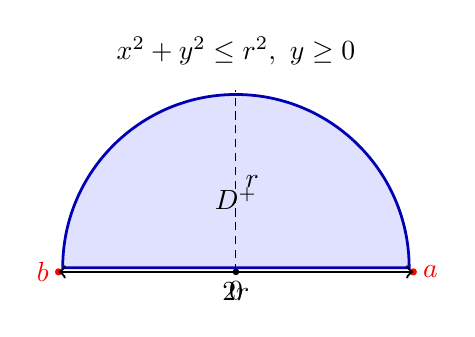
\begin{tikzpicture}
  \node[semicircle,draw=blue!70!black,fill=blue!12,line width=1pt,
    minimum width=44mm,minimum height=22mm,outer sep=1.5pt] (domain) at (0,0) {$D^+$};

  \fill[red] (domain.arc start) circle (1.3pt) node[right] {$a$};
  \fill[red] (domain.arc end) circle (1.3pt) node[left] {$b$};
  \fill[black] (domain.chord center) circle (1.2pt) node[below] {$0$};
  \draw[<->,thick] (domain.arc end) -- node[below] {$2r$} (domain.arc start);
  \draw[densely dashed] (domain.chord center) -- node[right] {$r$} (domain.apex);
  \node[above=2mm] at (domain.apex) {$x^2+y^2\le r^2,\ y\ge0$};
\end{tikzpicture}
\end{document}
